\subsection{Visualising Process Model Forecasts}\label{sec:visualisation}

In~\Cref{sec:experiment} we evaluated forecasting results, ensuring the relevance of the predicted process models. To that end, gaining actual insights from such predicted data remains a difficult task for the analyst. This section sets off to present the implementation of a novel visualization system to aid analysts in exploration of the event logs. The process of designing and implementing the system started by designing several prototypes that undergone rounds of discussions to mature into the implemented visualization system. 

The design of the PCE system is shown in Figure~\ref{fig:vis-two-brushes}. It shows an interactive visualization system with several connected views. The system is implemented with D3.js JavaScript library and is available at~\footnote{\url{google.com}}.


\begin{figure}
	\centering
	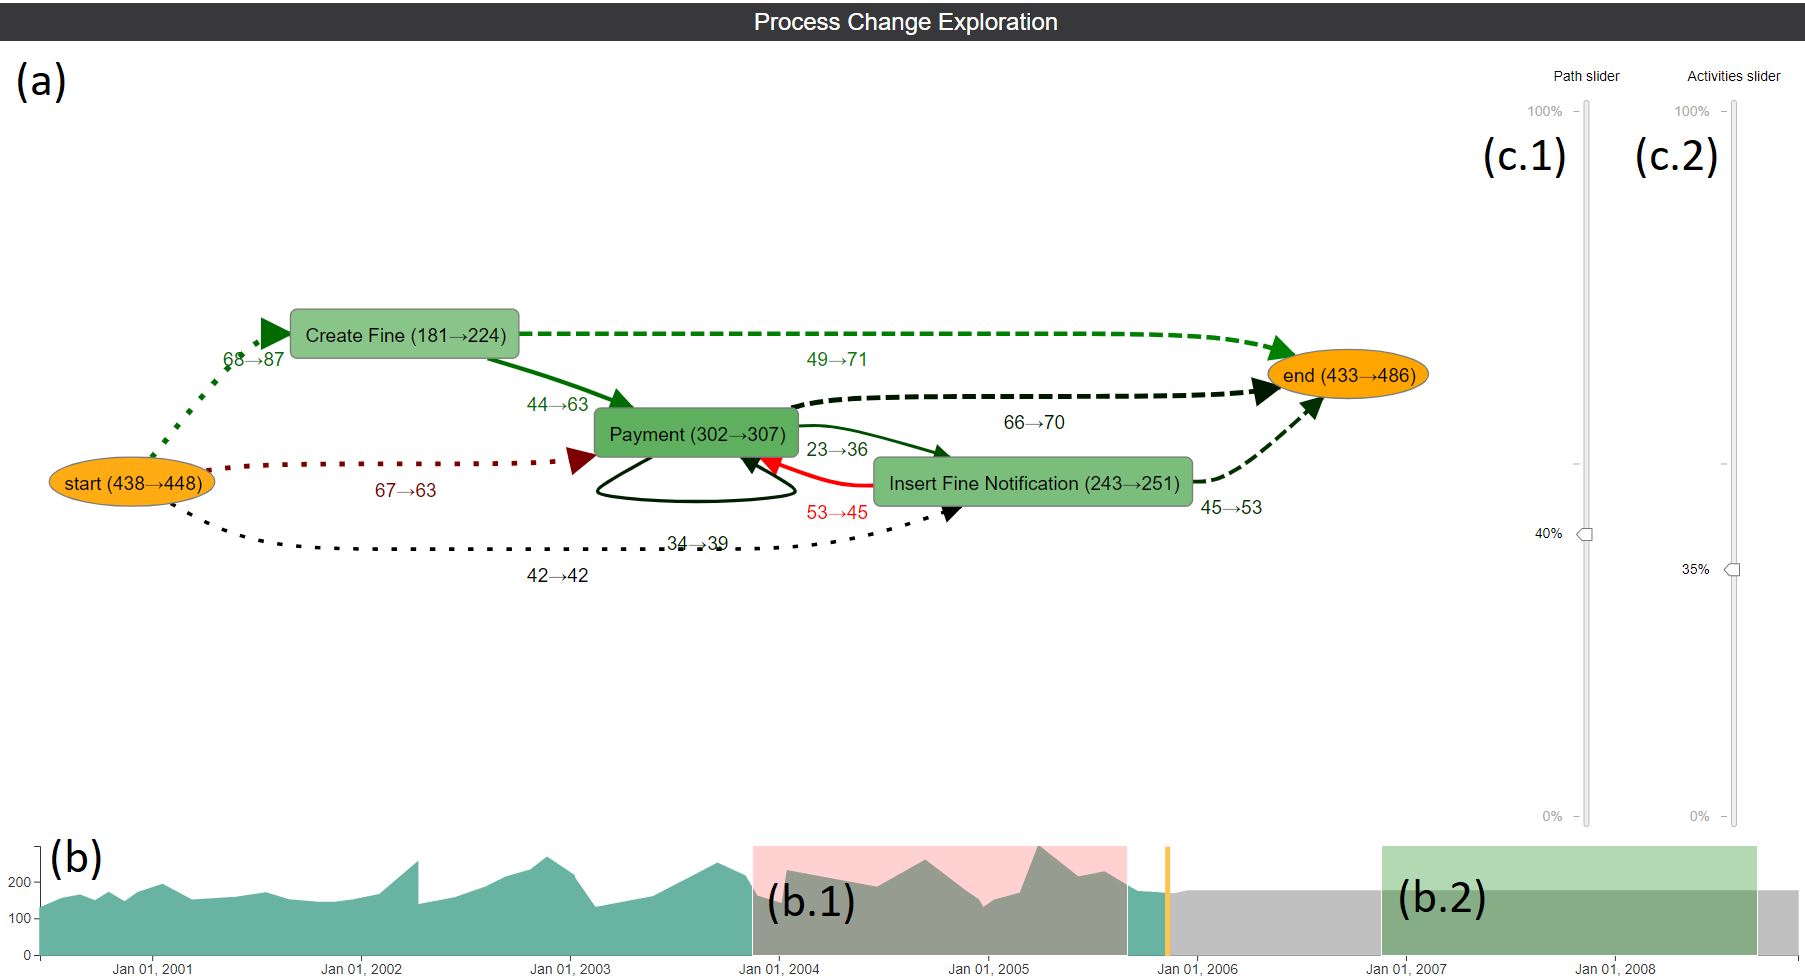
\includegraphics[width=\textwidth]{img/vis/actual-predicted-two-brushed-regions-system.PNG}
	\caption{Process Change Exploration (PCE) system.~\emph{(a)} shows~\emph{Adaptation Directly-Follows Graph (aDFG)} view.~\emph{(b)} shows the \emph{Timeline view with brushed regions} view. Users can brush one or more regions on this graph in order to filter the scope of the analysis~\emph{(b.1}, and~\emph{b.2)}. Two additional views~\emph{(c.1)}, and~\emph{(c.2)} show the \emph{activity and path sliders}.} 
	\label{fig:vis-two-brushes}
\end{figure}